\documentclass[12pt, a4paper, oneside]{ctexbook}
        \usepackage{amsmath, amsthm, amssymb, amsfonts, bm, graphicx, hyperref, mathrsfs}
        \usepackage{tcolorbox}
        \usepackage{tikz, xcolor, environ, xparse, zhnumber}
        
        %设置页眉
        \usepackage{fancyhdr}
        \pagestyle{fancy}
        
        
        
        
        
        
        \usetikzlibrary{shapes, decorations}
        
        %定义颜色
        \definecolor{dedcol}{RGB}{150,150,30}%推论环境的主色
        \definecolor{theocol}{RGB}{40,150,30}%定力环境的主色
        \definecolor{thrmcol}{RGB}{18,29,80}%默认定理等环境的背景色
        \definecolor{thrmedge}{RGB}{12,133,211}%默认定理等环境的边界颜色
        \definecolor{hyperlinkcol}{RGB}{32,112,102}%链接颜色
        \definecolor{hyperfilecol}{RGB}{135,206,235}%文件颜色
        \definecolor{hyperurlcol}{RGB}{3,168,158}%网址颜色
        \definecolor{hypercitecol}{RGB}{150,140,130}%引用颜色
        \definecolor{hlback}{RGB}{207,255,207}%高亮颜色
        \definecolor{opcol}{RGB}{235,125,75}%op颜色
        \definecolor{facecol}{RGB}{122,180,245}%封面颜色
        \definecolor{pscol}{RGB}{44,80,99}%图案颜色
        
        %定义hyper的颜色
        \hypersetup{
          colorlinks=true,
          linkcolor=hyperlinkcol,
          filecolor=hyperfilecol,
          urlcolor=hyperurlcol,
          citecolor=hypercitecol,
        }
        
        %定义字体
        \setCJKfamilyfont{hwxk}{华文行楷}
        \newcommand{\huawenxingkai}{\CJKfamily{hwxk}}
        \setCJKfamilyfont{hwkt}{华文楷体}
        \newcommand{\huawenkaiti}{\CJKfamily{hwkt}}
        \setCJKfamilyfont{hwhp}{华文琥珀}
        \newcommand{\huawenhupo}{\CJKfamily{hwhp}}
        \setCJKfamilyfont{hwls}{华文隶书}
        \newcommand{\huawenlishu}{\CJKfamily{hwls}}
        \setmainfont{华文楷体}
        
        %定义高亮
        \newtcbox{\hlbox}[1][red]{on line, arc = 2pt, outer arc = 0pt,
          colback = hlback, colframe = #1!50!black,
          boxsep = 0pt, left = 1pt, right = 1pt, top = 2pt, bottom = 2pt,
          boxrule = 0pt, bottomrule = 1pt, toprule = 1pt}
        \newcommand{\hl}[1]{\hlbox{#1}}
        \newcommand{\optxt}[1]{\textcolor{opcol}{#1}}
        
        
        
        
        
        %定义公式环境
        \newcommand{\newfancytheoremstyle}[5]{%
          \tikzset{#1/.style={draw=#3, fill=#2,very thick,rectangle,
              rounded corners, inner sep=10pt, inner ysep=20pt}}
          \tikzset{#1title/.style={fill=#3, text=#2}}
          \expandafter\def\csname #1headstyle\endcsname{#4}
          \expandafter\def\csname #1bodystyle\endcsname{#5}
        }
        
        \newfancytheoremstyle{fancythrm}{thrmcol!5}{thrmedge}{\huawenhupo}{\huawenxingkai}
        
        \makeatletter
        \DeclareDocumentCommand{\newfancytheorem}{ O{\@empty} m m m O{fancythrm} }{
          %% 定义计数器
          \ifx#1\@empty
            \newcounter{#2}
          \else
            \newcounter{#2}[#1]
            \numberwithin{#2}{#1}
          \fi
          %% 定义 "newthem" 环境
          \NewEnviron{#2}[1][{}]{%
            \noindent\centering
            \begin{tikzpicture}
              \node[#5] (box){
                \begin{minipage}{0.93\columnwidth}
                  \csname #5bodystyle\endcsname \BODY~##1
                \end{minipage}};
              \node[#5title, right=10pt] at (box.north west){
                {\csname #5headstyle\endcsname #3 \stepcounter{#2}\csname the#2\endcsname\; ##1}};
              \node[#5title, rounded corners] at (box.east) {#4};
            \end{tikzpicture}
          }[\par\vspace{.5\baselineskip}]
        }
        
        
        \makeatother
        
         % 定义各个环境的的样式
         % \newfancytheoremstyle{<name>}{inner color}{outer color}{head style}{body style}
        \newfancytheoremstyle{fancytheo}{theocol!5}{theocol}{\huawenhupo}{\huawenxingkai}
        \newfancytheoremstyle{fancyded}{dedcol!5}{dedcol}{\huawenhupo}{\huawenxingkai}
        
         % 定义各个新环境
         % \newfancytheorem[<number within>]{<name>}{<head>}{<symbol>}[<style>]
        \newfancytheorem[chapter]{define}{定义}{$\clubsuit$}
        \newfancytheorem[section]{deduce}{推论}{$\heartsuit$}[fancyded]
        \newfancytheorem[section]{theorem}{定理}{$\spadesuit$}[fancytheo]
        
        \title{{\Huge{量子计算机}}}
        \author{wave}
        \date{\today}
        \linespread{1.5}
        
        %设置章节标题样式\usepackage[english]{babel}
        \usepackage{blindtext}
        
        \usepackage[sc,compact,explicit]{titlesec} % Titlesec for configuring the header
        
        
        \usepackage{auto-pst-pdf} % Vectorian 装饰图案的 XeTeX 辅助 (见: https://tex.stackexchange.com/questions/253477/how-to-use-psvectorian-with-pdflatex)
        \usepackage{psvectorian} % Vectorian 中的装饰图案
        
        \let\clipbox\relax % PSTricks 已经定义了 \clipbox, 所以要去掉
        \usepackage{adjustbox} % 调整图案大小的
        
        \newcommand{\otherfancydraw}{% 定义图案
        \begin{adjustbox}{max height=0.5\baselineskip}% 根据行距设定高度,自己定
          \raisebox{-0.25\baselineskip}{
          \rotatebox[origin=c]{0}{% 旋转,自己定
            \psvectorian{84}% 图案,编号见 (http://melusine.eu.org/syracuse/pstricks/vectorian/psvectorian.pdf)
          }}%
        \end{adjustbox}%
        }
        
        % 画一条中间为图案的线 (见: https://tex.stackexchange.com/questions/15119/draw-horizontal-line-left-and-right-of-some-text-a-single-line/15122#15122)
        \newcommand*\ruleline[1]{\par\noindent\raisebox{.8ex}{\makebox[\linewidth]{\hrulefill\hspace{1ex}\raisebox{-.8ex}{#1}\hspace{1ex}\hrulefill}}}
        
        \titleformat% Formatting the header
          {\chapter} % command
          [block] % shape - Only managed to get it working with block
          {\normalfont\huawenlishu\huge} % format - Change here as needed
          {\centering 第\zhnum{chapter}章\\ \vspace{-0.6em}} % The Chapter N° label
          {0pt} % sep
          {\centering \ruleline{\otherfancydraw}\\ \vspace{-0.6em} % The horizontal rule
          \centering #1} % And the actual title
        
          \titleformat{\section}[block]{\huawenlishu\Large}{\thesection}{0pt}{\centering #1}

        %更改autoref的形式
        \def\equationautorefname{式}
        \def\footnoteautorefname{脚注}
        \def\itemautorefname{项}
        \def\figureautorefname{图}
        \def\tableautorefname{表}
        \def\appendixautorefname{附录}
        \def\chapterautorefname{章}
        \def\sectionautorefname{小节}
        \def\theoremautorefname{定理}

        
        
        
        \newcommand{\xkuo}[1]{\left(#1\right)}
        \newcommand{\dkuo}[1]{\left\lbrace#1\right\rbrace}
        \newcommand{\akuo}[1]{\left[#1\right]}
        \newcommand{\jkuo}[1]{\left\langle#1\right\rangle}
        \newcommand{\daa}[1]{\par\textcolor{blue}{\huawenxingkai #1}}
        \newcommand{\wen}[1]{\mbox{#1}}
        \newcommand{\you}{\mbox{又}}
        \newcommand{\dang}{\mbox{当}}
        \newcommand{\yyou}{\mbox{有}}
        \newcommand{\qie}{\mbox{且}}
        \newcommand{\jishu}[2]{\sum #1_n(#2)}
        \newcommand{\jjishu}[2][x]{\sum |#2_n(#1)|}
        \newcommand{\xti}[3]{\[(#1)#2\]\da{#3}}
        \newcommand{\pian}[2]{\frac{\partial #1}{\partial #2}}
        \newcommand{\ppian}[2]{\frac{\partial^2 #1}{\partial #2^2}}
        \newcommand{\dao}[2]{\frac{d#1}{d#2}}
        \newcommand{\ddao}[2]{\frac{d^2#1}{d#2^2}}
        \newcommand{\cen}{^\circ C}
        \newcommand{\fah}{^\circ F}
        \newcommand{\ji}[2]{\int_{#1}^{#2}}
        \newcommand{\qh}[1]{\sum\limits_{#1}}
        \newcommand{\jji}[1]{\iint\limits_{#1}}
        \newcommand{\ppi}{\frac\pi2}
        \newcommand{\ege}{\frac{\sqrt2}{2}}
        \newcommand{\e}[1]{\times10^{#1}}
        \newcommand{\ti}[1]{\textbf{#1}}
        
        
        \newcommand{\ldotfill}[2]{\leavevmode\xleaders\hbox{\rule{2pt}{0.4pt}\ }\hfill\null}
        
        %作业用
        \newcounter{que}
        \setcounter{que}{1}
        \newenvironment{question}[1][\theque]{\vspace*{2cm}\par\noindent\hrule\vspace*{2pt}\hrule\vspace*{10pt}\noindent\bfseries\large Ex#1.}{\stepcounter{que}}
        \definecolor{anscolor}{RGB}{50,120,170}
        \newenvironment{answer}[1][答]{\par\centerline{\makebox[10cm]{\dotfill}}\par\hangafter1\hangindent2em\noindent\textbf{#1.}\huawenxingkai\color{anscolor}\\}{\par}
        
        %数学分析
        \newcommand{\ya}[4]{\frac{\partial(#1,#2)}{\partial(#3,#4)}}
        \newcommand{\zkya}[4]{\pd #1#3#4\pd #2#4#3-\pd #1#4#3\pd #2#3#4}
        
        %复变函数
        \newcommand{\wqji}{\int_{-\infty}^{\infty}}
        
        %热学
        \newcommand{\pd}[3]{\xkuo{\frac{\partial#1}{\partial#2}}_#3}
        
        %原子物理
        \newcommand{\bra}[1]{\left\langle #1 \right|}
        \newcommand{\ket}[1]{\left| #1 \right\rangle}
        \newcommand{\p}[1]{\partial_{#1}}%对下标的偏导
        \newcommand{\ep}[1]{\epsilon_{#1}}%全反对称张量
        \newcommand{\dt}[1]{\delta_{#1}}%delta张量
        
        %理论力学
        \newcommand{\keq}[2]{\pian{\mathscr{#1}}{#2}}
        \newcommand{\zkps}[3]{\pian{#1}{q_#3}\pian{#2}{p_#3}-\pian{#1}{p_#3}\pian{#2}{q_#3}}
        
        %正文
        \newcommand{\sub}[1]{\(_{#1}\)}
        \newcommand{\sps}[1]{\(^{#1}\)}
        
        
        \begin{document}
          \renewcommand*{\psvectorianDefaultColor}{pscol}%设定图案颜色
        
          %
            \maketitle
        
            \pagenumbering{roman}
            \setcounter{page}{1}
        
            \begin{center}
                \Huge\huawenlishu{前言}
            \end{center}~\
        
            这是笔记的前言部分.
            ~\\
            \begin{flushright}
                \begin{tabular}{c}
                    何逸阳 \\
                    \today
                \end{tabular}
            \end{flushright}
            \begin{center}
                \Huge\huawenlishu{符号说明}
            \end{center}~\
        
            量子比特=量子位
        
            \newpage
            \pagenumbering{alph}
            \setcounter{page}{1}
            \tableofcontents
            \newpage
            \setcounter{page}{1}
            \pagenumbering{arabic}
        
            \chapter{量子电路}
        
            \begin{theorem}
                量子电路的哈密顿量:
                \begin{equation}
                    H=4E_Cn^2+\frac12E_L\phi^2
                \end{equation}
                (\(E_C\)前面的因子4是一个历史遗留)其中
                \begin{align}
                    \phi&=2\pi\frac{\Phi}{\Phi_0}&&\text{是约化的通量,表示电感中的“规范不变相位”}\\
                    n&=\frac{Q}{2e}&&\text{是容器内多的库珀对数量}\\
                    E_C&=\frac{e^2}{2C}&&\text{是使每个库珀对进入容器的能量}\\
                    E_L&=\xkuo{\frac{\Phi_0}{2\pi}}^2\cdot\frac1L&&\text{是电感能}\\
                    \Phi_0&=\frac{h}{2e}&&\text{是超导磁通量子}
                \end{align}
                此哈密顿量与描述一维二次势中的粒子,即量子谐振子(QHO)的哈密顿量相同。势能的函数形式影响本征解
            \end{theorem}
            \begin{theorem}
                算子\(n,\phi\)形成共轭对:
                \begin{equation}
                    \akuo{\phi,n}=i
                \end{equation}
            \end{theorem}
            \begin{theorem}
                该本征值问题的解给出了本征态的无穷列\(\dkuo{\ket{k}}\),其对应的本征能量\(E_k\)是等距的:
                \begin{equation}
                    E_{k+1}-E_k=\hslash\omega_r,\,\,\omega_r=\sqrt{8 E_L E_C} / \hbar=1 / \sqrt{L C}
                \end{equation}
                如图:

                \centering
                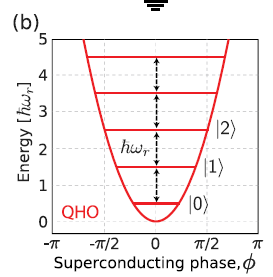
\includegraphics[width=0.4\textwidth]{scr/本征解.png}
            \end{theorem}
            \begin{theorem}
                我们可以用量子谐振子(QHO)哈密顿量更紧凑的形式(二次量化)表示这些结果:
                \begin{equation}
                    H=\hslash \omega_r\left(a^{\dagger} a+\frac{1}{2}\right)
                \end{equation}
                其中\(a^{\dagger}/a\)谐振腔单一激发的产生/湮灭算符

                我们将哈密顿量除去\(\hslash\),这样其单位就变成了角频率

                原来的电荷数和相位算符可表示为$n=n_{\mathrm{zpf}} \times i\left(a-a^{\dagger}\right)$ 以及 $\phi=\phi_{\mathrm{zpf}} \times\left(a+a^{\dagger}\right)$, 其中 $n_{\text {zpf }}=\left[E_L /\left(32 E_C\right)\right]^{1 / 4}$ 、 $\phi_{\text {pf }}=\left(2 E_C / E_L\right)^{1 / 4}$ 分别为电荷和相位变量的“零点波动”。
            \end{theorem}
            \begin{theorem}
              为防止出现不在计算内的量子态,我们需要给我们的系统添加非谐振(或者非线性)部分。简而言之,各个态之间的转换频率要有足够的差异性,以便能够单独寻址。非谐波的数量限制了用于驱动量子比特的脉冲的长度。

              为了引入非线性部分,我们使用\hl{约瑟夫逊结}(一个非线性、无损耗的电路元件)作为超导电路中的骨干:我们将QHO的\hl{线性电感替换为约瑟夫逊结},成为非线性电感的角色。于是我们通过约瑟夫森效应的关系式计算得到新的势能函数形式后,可以求得修正的哈密顿量形式:
              \begin{equation}
                H=4E_cn^2-E_J\cos(\phi)
              \end{equation}
              其中\(E_C=e^2 /\left(2 C_{\Sigma}\right), C_{\Sigma}=C_s+C_J\)是总电容,包括分流电容\(C_s\)和结自带的电容\(C_J\);\(E_J=\frac{I_c\Phi_0}{2\pi}\)为约瑟夫森能量。

              如图:

              \centering 
              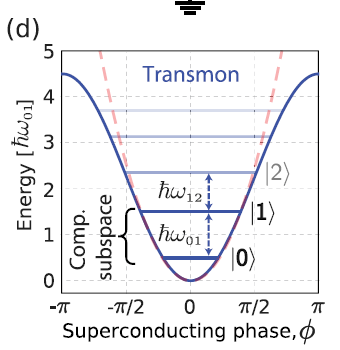
\includegraphics[width=0.4\textwidth]{scr/本征解非线性.png}
            \end{theorem}
            \begin{theorem}
              系统的动力学由\(\frac{E_c}{E_J}\)主导。当\(E_J\leqslant E_c\)时,量子比特变得对电荷噪声高度敏感,使其很难实现高相干性。为了使得\(E_J\gg E_c\),我们通过用大电容来分流结,使\(E_c\)变小(\(C_s\gg C_J\))。这个电路的量子比特通常被称为\hl{transmon(跨频)量子比特}。

              在这个限制下,超导相\(\phi\)是一个很好的量子数,即由量子波函数表示的\(\phi\)值的扩散(或量子涨落)很小。因此,低能本征态近似为势阱中的局域态。

              我们将哈密顿的势能项幂级数展开:
              \begin{equation}
                E_J \cos (\phi)=\frac{1}{2} E_J \phi^2-\frac{1}{24} E_J \phi^4+\mathcal{O}\left(\phi^6\right)
              \end{equation}
              其中主导的二次项与原来的QHO势能项一致,而四次项则改变了本征解并破坏了原本的谐波能量结构。
              
              注意,四次项的负系数表示非谐系数\(\alpha=\omega_{\mathrm{q}}^{1 \rightarrow 2}-\omega_{\mathrm{q}}^{0 \rightarrow 1}\)小于零。因此,它的上极限不能是任意大。

              对于transmon的例子,\(\alpha=-E_c\)一般被设置为100-300MHz,以保持一个理想的量子比特频率\(\omega_q=\frac{\sqrt[]{8E_JE_c}-E_c}{\hslash}=\)3-6GHz,同时保持一个足够大的\(\frac{E_J}{E_c}\)来抑制

              (由于电荷灵敏度被指数级抑制的同时非谐性的减少仅按幂次的速度,这允许我们做出一个可行的器件。)

            \end{theorem}
            \begin{theorem}
              只包括到四阶项的哈密顿量类似于Duffing振荡器
              \begin{equation}
                H=\omega_{\mathrm{q}} a^{\dagger} a+\frac{\alpha}{2} a^{\dagger} a^{\dagger} a a
              \end{equation}
              由于\(|\alpha|\ll\omega_q\)我们可以看到transmon量子比特基本上是一个弱非谐的振子(AHO)。

              如果激发到更高的非计算态在某个电路门中被抑制,要么是由于足够大的\(|\alpha|\),要么是由于鲁棒控制技术比如绝热门(DRAG)脉冲技术

              我们现在可以有效地将AHO看作一个量子两能级系统,将哈密顿量简化为(我们应该始终记住,物理上存在更高的能级,并在设计系统及其控制过程时,应考虑到它们对系统动力学的影响。事实上,更高的能级已被证明可以实现更效率的门电路)
              \begin{equation}
                H=\omega_{\mathrm{q}} \frac{\sigma_z}{2}
              \end{equation}
              其中\(\sigma_z\)是泡利算符的z分量
            \end{theorem}

            \begin{theorem}
              除了减少电荷分散,使用一个大的分流电容器还有一个好处就是使我们能够规划量子系统的电场分布,从而规划表面损失机制。在开发3维transmon(比如将二维跨频耦合到三维腔)时,当我们使两个横向电容板之间的间隙很大(与膜厚相比),那么由于一小部分电场与有损耗的界面相互作用(比如金属-衬底和衬底-真空界面,已经被广泛研究),相干时间增加。
            \end{theorem}

            \subsection{可调谐量子比特:分裂transmon}
            \begin{theorem}
              为了实现高保真的快速门操作,正如实现量子逻辑所需要的那样,今天实现的许多(尽管不是全部)量子处理器架构都具有可调谐的量子位频率。

              例如,在某些情况下,我们需要将两个量子位带入共振来交换能量,同时我们还需要能够在空闲期间将它们分离,以最小化它们的相互作用。要做到这一点,我们需要一个外部参数,它允许我们以可控的方式访问系统的一个自由度。

              一种广泛应用的技术是用一个由两个相同结中断的环来取代单个约瑟夫森结——形成直流超导量子干涉装置(DC- squid)。

              由于squid的两臂之间存在干扰,可以通过施加穿过环路的磁通来降低两个并联接点的有效临界电流

              由于磁通的量子化条件,回路上所有感性的元件的通量之和加上外部施加磁通等于一个整数倍的超导通量子:
              \begin{equation}
                \varphi_1-\varphi_2+2 \varphi_e=2 \pi k
              \end{equation}
              其中\(\varphi_e=\pi \frac{\Phi_{ext}}{\Phi_0}\)

              利用这一条件,我们可以消除一个自由度,并将SQUID-loop视为单结,但有一个重要的变化,即\(E_J\)可以通过外部通量\(\Phi_{ext}\)(通过SQUID临界电流)调节。

              分裂transmon量子的有效哈密顿量(忽略常数)是
              \begin{equation}\label{eqn:symtransmonH}
                H=4 E_C n^2-\underbrace{2 E_J\left|\cos \left(\varphi_e\right)\right|}_{E_J^{\prime}\left(\varphi_e\right)} \cos (\phi) .
              \end{equation}

              可以看出,量子比特的频率能够用\(\Phi_{ext}\)周期性地调节
            \end{theorem}

            \begin{theorem}
              虽然分裂transmon可以通过外部磁场调谐频率,但它也导致了对随机磁通波动的敏感性,称为磁通噪声。量子比特频谱的斜率\(\pian{\omega_q}{\Phi_{ext}}\),表明了通量噪声对量子比特频率的一阶影响有多强(除了在\(\Phi_{ext}=k\Phi_0\)的地方\(\pian{\omega_q}{\Phi_{ext}}=0\)以外,其它地方的敏感程度均非零)。

              最近的一项进展集中在降低量子比特对通量噪声的敏感性,同时保持足够的可调性来操作我们的量子门。其思想是使分裂跨子中的两个连接不对称,
              如图:

              \begin{center}
              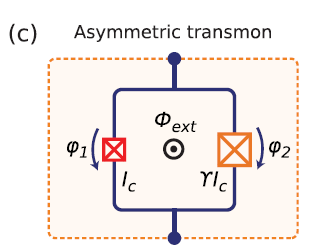
\includegraphics[width=0.3\textwidth]{scr/不对称transmon.png}
              \end{center}
              
              其哈密顿量为:
              \begin{equation}
                H=4 E_C n^2-\underbrace{E_{J \Sigma} \sqrt{\cos ^2\left(\varphi_e\right)+d^2 \sin ^2\left(\varphi_e\right)}}_{E_J^{\prime}\left(\varphi_e\right)} \cos (\phi)
              \end{equation}
              其中\(E_{J \Sigma}=E_{J 1}+E_{J 2} \text { , } d=(\gamma-1) /(\gamma+1)\)是结不对称参数。我们可以将两个结视为一个单结跨子,具有的有效约瑟夫森能量\(E_J'(\varphi_e)\)。当d等于0时,它退化为\autoref{eqn:symtransmonH}(\(E_J^{\prime}\left(\varphi_e\right)=E_{J \Sigma}\left|\cos \left(\varphi_e\right)\right|=2E_{J}\left|\cos \left(\varphi_e\right)\right|\))


              
            \end{theorem}

            \begin{theorem}
              不对称情况下,通量灵敏度在整个可调谐频率范围内被抑制。因此,通过使用非对称跨频,引入了一个小的频率调谐范围,足以补偿制造的变化,而不会引入不必要的大通量噪声敏感性,从而保持高相干性。
              
              另一个例子是基于绝热控制相位的表面编码方案(CPHASE门)需要量子位之间特定的频率配置,以避免频率拥挤的问题,而非对称transmons很好地符合其良好的频率范围。

              总的来说,随着量子处理器规模的扩大和制造工艺的改进,未来非对称transmons很可能有更广泛的应用。
            \end{theorem}

            \subsection{更大的非谐性:通量量子比特(flux qubit)和fluxonium}

            \begin{theorem}
              分裂transmon,无论它是否对称,都与单结版本共享相同的拓扑结构,产生正弦势。因此,这些量子位的特性在多大程度上可以被改造,并没有从根本上改变。特别是,跨声门型量子位的有限非谐性本质上导致了对更高能量态的显著剩余激励,破坏了门操作的性能。为了超越这一点,有必要在电路中引入额外的复杂性。
            \end{theorem}
            \begin{theorem}
              一个方法是通量量子比特的方式,其环路有三、四个结。在其中一个分支上有一个较小的结;而在另一个分支上有两个相同的结,都是小结的\(\gamma\)倍。与分裂跨通相比,多增加一个结是非常重要的,因为它改变了电路拓扑结构并重塑了势能分布。
            \end{theorem}
            \begin{theorem}
              由于\(\gamma>1\),通常我们可以近似把这个问题看作一个在准一维势中运动的粒子。这种近似下,其\hl{哈密顿量}为
              \begin{equation}
                H \approx 4 E_C n^2-E_J \cos \left(2 \phi+\varphi_e\right)-2 \gamma E_J \cos (\phi)
              \end{equation}
              其中,相位是两个结的相位之和:\(\phi=\frac12(\varphi_1+\varphi_2)\)(假设两个结的电流方向相同)。第二项是小结的约瑟夫森能量\(E_J\)。第三项对应两个结总共\(2\gamma E_J\)的能量。这两项和的势分布及相应本征态均取决于外部通量\(\varphi_e\)以及比率\(\gamma\)。当半个超导通量量子(superconducting flux quantum)穿过量子比特电路时,在此通量偏点(flux bias point),量子位频谱(spectrum)达到最小值,量子位频率对通量噪声一阶不敏感。
            \end{theorem}
            \begin{theorem}
              当\(\varphi_e=\pi+2k\pi,\,k\in\mathbb Z\)时,量子位频谱达到最小值,量子位频率对通量噪声一阶不敏感。这个点通常被称为“通量简并点”,在这个点上通量量子比特往往具有最佳相干时间,因此常常作为工作点。这时的势能可以当做单井\((\gamma\geq 2)\)或者双井\((\gamma<2)\)。单井情况与transmon量子位有一些相似之处,其中哈密顿量的二次项和四次项分别决定了谐性和非谐性。
            \end{theorem}

            \begin{theorem}
              电容分流通量量子位(CSFQ)表现出长相干性和相当高的非谐性,与transmon量子比特相反,CSFQ的非谐性是正的。

              基于循环电流状态——持续电流通量量子位(PCFQ)——的直观图像给出了一个令人满意的量子比特自由度的物理描述。PCFQ最重要的特征是它的非谐性可以比transmon、CSFQ大得多;其跃迁矩阵元素\(|\langle 1|\hat{n}| 0\rangle|,|\langle 1|\hat{\phi}| 0\rangle|\)变得更小,因此,可以保持更长的relaxation time。这些特征在与它类似的fluxonium量子比特中更明显。
            \end{theorem}
            \begin{theorem}
              通量量子的例子说明了如何通过选择各种电路参数来设计量子位的特性,结和随之而来的双谐波轮廓的引入。这一想法的延伸是fluxonium量子位,它能够通过设计跃迁矩阵实现毫秒\(T_1\)时间,部分原因是适用于这种保护良好的量子位的新型门方案的发明
            \end{theorem}

            \chapter{噪声}

            \section{噪声模型和退相干}
            \subsection{布洛赫球(Bloch Sphere)}\
            \begin{define}
              “布洛赫球”是一个单位球,用来表示两能级系统的量子态。终点在球面上的“Bloch向量”表示状态\(\ket{\psi}=\alpha\ket0+\beta\ket1\)。
              一般来讲,Bloch球的北极代表状态\(\ket0\),南极代表状态\(\ket1\)。


              连接南北两极的z轴被称为
              “纵向轴”,表示量子比特特征态中状态\(\ket0\)和\(\ket1\)的“量化轴”。此外,x - y平面称为“横轴平面”。在这个笛卡尔坐标系中,单位布洛赫向量\(\vec a=(\sin\theta\cos\varphi,\sin\theta\sin\varphi,\cos\theta)\)。按照我们的惯例,在北极的状态j0i与þ1相关,而在南极的状态\(\ket1\)与-1相关。
            \end{define}
        
        
        \end{document}